\documentclass[12pt]{article}
%\usepackage[margin=1in]{geometry}% Change the margins here if you wish.
%\setlength{\parindent}{0pt} % This is the set the indent length for new paragraphs, change if you want.
%\setlength{\parskip}{5pt} % This sets the distance between paragraphs, which will be used anytime you have a blank line in your LaTeX code.
%\pagenumbering{gobble}% This means the page will not be numbered. You can comment it out if you like page numbers.

%------------------------------------

\usepackage{color}
\usepackage[utf8]{inputenc}
\usepackage{hyperref}
\usepackage{listings}% http://ctan.org/pkg/listings

\usepackage[margin=1in]{geometry}
\usepackage{cprotect}
\usepackage{mathtools}
\usepackage{fancyvrb}

\usepackage{comment}
\linespread{1.6}
\usepackage{examplep}

\renewcommand{\refname}{Referências}

% These packages allow the most of the common "mathly things"
\usepackage{amsmath,amsthm,amssymb}

% This package allows you to add images.
\usepackage{graphicx}
\usepackage{float}

\usepackage{listings}
\usepackage{upquote,textcomp}

\newcommand{\blu}{\textcolor{blue}}
\newcommand{\red}{\textcolor{red}}
\newcommand\todo[1]{\red{\Large \text{TODO: #1}}}

\newcommand{\defeq}{\vcentcolon=}
\newcommand{\eqdef}{=\vcentcolon}
\newcommand\Item[1][]{%
  \ifx\relax#1\relax  \item \else \item[#1] \fi
  \abovedisplayskip=0pt\abovedisplayshortskip=0pt~\vspace*{-\baselineskip}}
\newcommand\eb[1]{[[\texttt{#1}]]}
% Should you need any additional packages, you can load them here. If you've looked up something (like on DeTeXify), it should specify if you need a special package.  Just copy and paste what is below, and put the package name in the { }.  
\usepackage{wasysym} %this lets me make smiley faces :-)

\title{CML - Uma Linguagem para {\it Machine Learning} \\ \Large Relatório 2 - Trabalho de Conceitos de Linguagem de Programação}

\author{Caio Lopes, Leonardo Blanger, Marcelo Silvarolla}

\date{16 de maio de 2018}

\begin{document}
\lstset{
  basicstyle=\ttfamily,
  columns=fullflexible,
  keepspaces=true,
  mathescape
}

\maketitle
\tableofcontents
\newpage
\section{Sintaxe Concreta}
Usamos a seguinte notação para nossas regras EBNF:
\begin{center}
\begin{tabular}{c c}
definição  : \\
concatenação  (espaço) \\
união  $\vert$  \\
agrupamento  ($\ldots$) \\
{\it string} terminal  \verb!"!$\ldots$\verb!"! \\
{\it string} terminal  '$\ldots$' \\
*  zero ou mais \\
+  um ou mais \\
/* $\ldots$ */  comentário \\
terminação  ;
\end{tabular}
\end{center}

O alfabeto, isto é, o conjunto de símbolos terminais da nossa linguagem, será o conjunto de caracteres ASCII, conforme a tabela:
\begin{center}
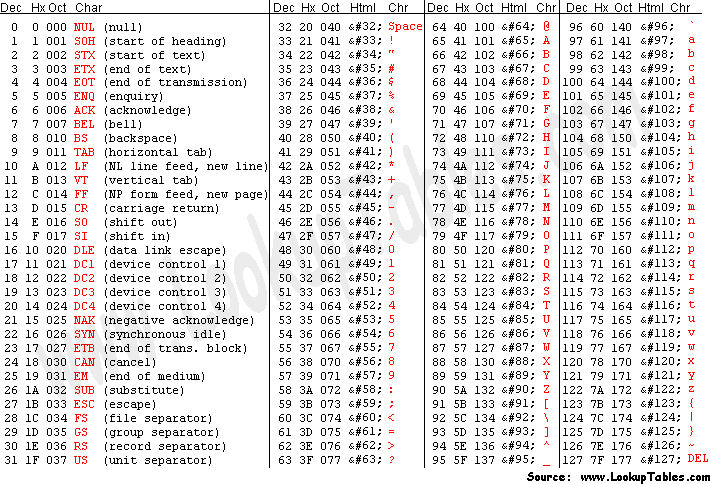
\includegraphics[width=\linewidth,height=\textheight,keepaspectratio]{asciitable.png}
\end{center}
\subsection{Palavras Reservadas}
{\tt char else real bool string dataset model if int return void while skip \\ || < <= > >= == != ; \{ \} , = ( ) [ ] ! - + * /}
\subsection{Regras Léxicas}
Os espaços são ignorados na análise léxica.
Denotaremos os {\it tokens} por seus nomes em LETRAS MAIÚSCULAS, para os diferenciar dos demais símbolos não-terminais.

\begin{verbatim}
D : "0" | "1" | "2" | "3" | "4" | "5" | "6" | "7" | "8" | "9";
L : "A" | "B" | "C" | "D" | "E" | "F" | "G"
       | "H" | "I" | "J" | "K" | "L" | "M" | "N"
       | "O" | "P" | "Q" | "R" | "S" | "T" | "U"
       | "V" | "W" | "X" | "Y" | "Z" | "a" | "b"
       | "c" | "d" | "e" | "f" | "g" | "h" | "i"
       | "j" | "k" | "l" | "m" | "n" | "o" | "p"
       | "q" | "r" | "s" | "t" | "u" | "v" | "w"
       | "x" | "y" | "z" | "_";
A : L | D;
ES : "\" ("'" | '"' | "\" | "n" | "t");
CHAR : "char";
ELSE : "else";
REAL : "real";
BOOL : "bool";
STRING : "string";
DATASET : "dataset";
MODEL : "model";
IF : "if";
INT : "int";
RETURN : "return";
VOID : "void";
WHILE : "while";
SKIP : "skip";
IDENTIFIER : L (A)*;
INT_LITERAL : (D)+;
REAL_LITERAL : (D)* "." (D)+ | (D)+ ".";
NONQUOTE_BACKSLASH_NEWLINE :
' ' | '!' | '"' | '#' | '$' | '%' | '' | "'" | '(' | ')' | 
'*' | '+' | ',' | '-' | '.' | '/' | '0' | '1' | '2' | '3' | 
'4' | '5' | '6' | '7' | '8' | '9' | ':' | ';' | '<' | '=' | 
'>' | '?' | '@' | 'A' | 'B' | 'C' | 'D' | 'E' | 'F' | 'G' | 
'H' | 'I' | 'J' | 'K' | 'L' | 'M' | 'N' | 'O' | 'P' | 'Q' | 
'R' | 'S' | 'T' | 'U' | 'V' | 'W' | 'X' | 'Y' | 'Z' | '[' | 
'\' | ']' | '^' | '_' | '`' | 'a' | 'b' | 'c' | 'd' | 'e' | 
'f' | 'g' | 'h' | 'i' | 'j' | 'k' | 'l' | 'm' | 'n' | 'o' | 
'p' | 'q' | 'r' | 's' | 't' | 'u' | 'v' | 'w' | 'x' | 'y' | 
'z' | '{' | '|' | '}' | '~';
CHAR_LITERAL : "'" (NONQUOTE_BACKSLASH_NEWLINE | '"' | ES)"'";
STRING_LITERAL : '"' (NONQUOTE_BACKSLASH_NEWLINE | "'" | ES)* '"';
AND_OP : "&&";
OR_OP : "||";
LE_OP : "<=";
GE_OP : ">=";
EQ_OP : "==";
NE_OP : "!=";
\end{verbatim}
\footnote{\texttt{D} de dígito, \texttt{L} de letra, \texttt{A} de alfanumérico (letra ou dígito), \texttt{ES} de {\it escape sequence}.  Note que incluímos o {\it underscore} como letra.

O não-terminal \texttt{NONQUOTE\_BACKSLASH\_NEWLINE} define o conjunto de todos os caracteres ASCII imprimíveis que não são uma aspa simples, aspa dupla, barra inversa ou quebra de linha.}

\subsection{Regras Sintáticas}
\subsubsection{Símbolos Terminais}
Os símbolos terminais na análise sintática são os {\it tokens} gerados na análise léxica acima.
\subsubsection{Expressões}
Os espaços são ignorados na análise léxica.
\begin{verbatim}
/* Expressões necessariamente "atômicas":
    Expressões que não causam ambiguidades quando dentro
    de uma expressão maior, mesmo quando a precedência
    das operações não é conhecida
    Estas expressões podem, portanto, ser pensadas
    como identificadores ou literais. */

primary_expression
    : IDENTIFIER
    | literal
    | '{' '}'
    | '{' expression_list '}'
    | '(' expression ')'
    | array_access
    | IDENTIFIER '(' ')'
    | IDENTIFIER '(' expression_list ')'
    ;

literal
    : INT_LITERAL
    | REAL_LITERAL
    | BOOL_LITERAL
    | CHAR_LITERAL
    | STRING_LITERAL
    ;

/* Expressões "não-atômicas" */
expression_list
    : expression
    | expression_list ',' expression
    ;

expression
    : logical_or_expression
    | IDENTIFIER '=' expression
    | array_access '=' expression
    ;

array_access
    : IDENTIFIER '[' expression ']'
    | array_access '[' expression ']'
    ;

logical_or_expression
    : logical_and_expression
    | logical_or_expression OR_OP logical_and_expression
    ;

logical_and_expression
    : relational_expression
    | logical_and_expression AND_OP relational_expression
    ;

relational_expression
    : additive_expression
    | additive_expression '<' additive_expression
    | additive_expression '>' additive_expression
    | additive_expression LE_OP additive_expression
    | additive_expression GE_OP additive_expression
    | additive_expression EQ_OP additive_expression
    | additive_expression NE_OP additive_expression
    ;

additive_expression
    : multiplicative_expression
    | additive_expression '+' multiplicative_expression
    | additive_expression '-' multiplicative_expression
    ;

multiplicative_expression
    : unary_minus_expression
    | multiplicative_expression '*' unary_minus_expression
    | multiplicative_expression '/' unary_minus_expression
    ;

unary_minus_expression
    : neg_expression
    | '-' neg_expression
    ;

neg_expression
    : primary_expression
    | '!' neg_expression
    ;
\end{verbatim}


\subsubsection{Comandos}
\begin{verbatim}
command
    : compound_command
    | expression_command
    | selection_command
    | iteration_command
    | jump_command
    | SKIP ';'
    ;

compound_command
    : '{' declaration_or_command_list '}'
    ;

declaration_or_command_list 
    : declaration_or_command
    | declaration_or_command_list declaration_or_command
    ;

declaration_or_command
    : declaration
    | command
    ;

expression_command
    : ';'
    | expression ';'
    ;

selection_command
    : IF '(' expression ')' compound_command ELSE compound_command
    | IF '(' expression ')' compound_command
    ;

iteration_command
    : WHILE '(' expression ')' command
    ;

jump_command
    : RETURN ';'
    | RETURN expression ';'
    ;
\end{verbatim}

\subsubsection{Declarações}
\begin{verbatim}
declaration
    : type_specifier IDENTIFIER ';'
    | type_specifier IDENTIFIER '=' expression ';'
    ;

parameter_declaration_list
    : parameter_declaration
    | parameter_declaration_list ',' parameter_declaration
    ;

parameter_declaration
    : type_specifier IDENTIFIER
    ;

type_specifier
    : VOID
    | CHAR
    | INT
    | REAL
    | BOOL
    | STRING
    | DATASET
    | MODEL
    | type_specifier '[' ']'
    ;
\end{verbatim}

\subsubsection{Definições}
\begin{verbatim}
function_definition
    : type_specifier IDENTIFIER '(' ')' compound_command
    | type_specifier IDENTIFIER '(' 
    | parameter_declaration_list ')' compound_command
    ;
\end{verbatim}

\subsubsection{Programa}
\begin{verbatim}
program
    : declaration_or_function_definition
    | program declaration_or_function_definition
    ;

declaration_or_function_definition
    : function_definition
    | declaration
    ;

\end{verbatim}


\subsection{Exemplo}

O exemplo a seguir ilustra o uso da linguagem para tentar predizer o resultado do oscar. Ele assume que exista uma planilha {\tt  movies.csv} no diretório atual, que possua uma lista de filmes, cada filme em uma linha, onde cada coluna assuma algum atributo dos filmes (bilheteria, diretor, duração, etc), e exista uma coluna {\tt hasWonOscar} indicando se o respectivo filme venceu o prêmio. O exemplo assume também que exista um outro arquivo {\tt moviesRevenue.csv} de filmes inéditos, onde exista as mesmas colunas que no arquivo anterior, com exceção da coluna ``hasWonOscar''.

O código abaixo carrega o primeiro arquivo, separa a coluna das saídas ({\tt y}) da matriz das entradas ({\tt X}), treina um modelo classificador do tipo {\it perceptron} nestes dados, e usa este modelo para predizer o resultado do oscar para os filmes do segundo arquivo.

\blu{Generalizamos as funções \texttt{load\_data} e \texttt{save\_data} para funcionarem com separadores arbitrários no arquivo CSV. No exemplo abaixo, usamos o caractere separador \texttt{','}. Também mudamos o nome das funções \texttt{remove\_cols} e \texttt{cols} para \texttt{remove\_columns} e \texttt{columns}.}

\begin{Verbatim}
dataset getRelevantMovies(dataset movies){
	int num_movies = num_rows(movies);
	if (num_movies < 10000){
		return movies;
	}
	else {
		return rows(movies, 0, 10000);
	}
}

int main(){
	string file_name = "movies.csv";
	dataset movies = load_data(file_name, ',');
	dataset top_movies = getRelevantMovies(movies);
	
	dataset X = remove_columns(top_movies, {"hasWonOscar"});
	dataset y = columns(top_movies, {"hasWonOscar"});
	model classifier = perceptron(X, y, 2000);
	
	dataset unclassified_movies = 
			load_data("moviesRevenue.csv", ',');
	dataset prediction = 
		predict(unclassified_movies, classifier);
	
	save_data(prediction, "oscarFavourites.csv", ',');
}
\end{Verbatim}



\section{Semântica}

\subsection{Domínios Sintáticos}

\begin{itemize}
\item {\tt Identifier $\defeq$} conjunto de todas as sequências finitas de terminais deriváveis a partir do não-terminal {\tt id} abaixo.

\item {\tt Literal $\defeq$} conjunto de todas as sequências finitas de terminais deriváveis a partir do não-terminal {\tt lit} abaixo.

\item {\tt ArrayAccess $\defeq$} conjunto de todas as sequências finitas de terminais deriváveis a partir do não-terminal {\tt arr\_access} abaixo.

\item {\tt Expression $\defeq$} conjunto de todas sequências finitas de terminais deriváveis a partir do não-terminal {\tt exp} abaixo.

\item {\tt ExpressionList $\defeq$} conjunto de todas sequências finitas de terminais deriváveis a partir do não-terminal {\tt exp\_list} abaixo.

\item {\tt Command $\defeq$} conjunto de todas as sequências finitas de terminais deriváveis a partir do não-terminal {\tt cmd} abaixo.

\item {\tt Declaration $\defeq$} conjunto de todas as sequências finitas de terminais deriváveis a partir do não-terminal {\tt dec} abaixo.

\item {\tt DeclarationOrCommandSequence $\defeq$} conjunto de todas as sequências finitas de terminais deriváveis a partir do não-terminal {\tt dec} ou do não-terminal {\tt cmd} abaixo.

\item {\tt Program $\defeq$} conjunto de todas as sequências finitas de terminais deriváveis a partir do não-terminal {\tt prog} abaixo.

\end{itemize}



\subsection{Sintaxe Abstrata}
A sintaxe em EBNF acima contém detalhes irrelevantes para a semântica, especificando formalmente a associatividade e precedência dos operadores. Aqui, apresentamos uma sintaxe simplificada, a sintaxe abstrata, que, apesar de ambígua, é suficiente para a definição da semântica. Estamos essencialmente seguindo o capítulo $9$ do livro de Kenneth Slonneger e Barry L. Kurtz "Formal Syntax and Semantics of Programming Languages" \cite{Chap9}.
Observe que \verb!IDENTIFIER! e \verb!literal! estão definidos na sintaxe concreta acima.
\subsubsection{Expressões}

\begin{verbatim}
id : IDENTIFIER;
lit : literal;
exp_list : exp | exp_list "," exp;
arr_access : id_or_arr_access "[" exp "]";
id_or_arr_access : id | id_or_arr_access "[" exp "]";
exp :lit | "{" "}" | "{ exp_list "}" |
     exp "||" exp | id_or_arr_access "=" exp | exp "&&" exp |
     exp "==" exp | exp "!=" exp | exp "<" exp | exp "<=" exp |
     exp ">" exp | exp ">=" exp | "-" exp | exp "+" exp |
     exp "-" exp | exp "*" exp | exp "/" exp |
     "(" exp ")" | id_or_arr_access | id "(" ")" |
     id "(" exp_list ")" | "!" exp;
\end{verbatim}

\subsubsection{Comandos}
\begin{verbatim}
cmd : comp_cmd | exp_cmd | 
       sel_cmd | iter_cmd |
       jump_cmd | SKIP ";";
dec_cmd = dec | cmd
dec_cmd_list = dec_cmd | dec_cmd_list dec_cmd
comp_cmd : "{" dec_cmd_list "}";
exp_cmd : exp ";";
sel_cmd : IF "(" exp ")" comp_cmd ELSE comp_cmd |
                 IF "(" exp ")" comp_cmd;
iter_cmd : WHILE "(" exp ")" cmd;
jump_cmd : RETURN ";" | RETURN exp ";";
\end{verbatim}

\subsubsection{Declarações}
Note que \verb!type_specifier! está definido na sintaxe concreta acima.
\begin{verbatim}
type_spec : type_specifier;
dec : type_spec id ";" | 
      type_spec id "=" exp ";";
\end{verbatim}

\subsubsection{Definições}

\begin{verbatim}
fun_def : type_spec id "(" ")" comp_cmd |
         type_spec id "(" param_dec_list ")" comp_cmd;
param_dec : type_spec id;
param_dec_list : param_dec | param_dec_list "," param_dec;
\end{verbatim}

\subsubsection{Programa}

\begin{verbatim}
prog : dec_or_fun_def | prog dec_or_fun_def;
dec_or_fun_def : fun_def | dec;
\end{verbatim}

\subsection{Domínios Semânticos}

Denotamos por $X \rightarrow Y$ o conjunto\footnote{Às vezes, como nas funções auxiliares init e last, utilizamos essas definições quando $X$ e $Y$ são classes próprias, o que obviamente não é problema.}de funções parciais de $X$ em $Y$, onde $X$ e $Y$ são conjuntos quaisquer. Escrevemos $f:X \rightarrow Y$ para dizer que $f$ é função parcial de $X$ em $Y$. Ademais, se $n\in\mathbb{N}$, $X^n \defeq X \times \ldots (n \text{ vezes }) \ldots \times X \defeq \{f \mid f \text{ é função total do conjunto } \{0, 1, \ldots, n-1\}\text{ em } X\}$ é o conjunto de tuplas (isto é, vetores) de $n$ elementos de $X$. Por exemplo, $\mathbb{R}\to\mathbb{R}$ é o conjunto de todas as funções da reta na reta, enquanto $\mathbb{R}^n$ é o espaço euclidiano $n$-dimensional.

\begin{itemize}
\item $Int \defeq \{\ldots, -2, -1, 0, 1, 2, \ldots\} = \mathbb{Z}$

\item $Real \defeq  \mathbb{R}$
\item $Bool \defeq \{true, false\}$
\item $Char \defeq \{0, \ldots, 127\}$, onde os números de 0 a 127 são interpretados conforme o padrão ASCII, e.g., 43 representa `$+$', 49 representa `1', etc. Para mais detalhes, ver tabela no início do relatório.

Definimos, para cada conjunto $X$, o conjunto $X[]$ dos vetores de elementos de $X$ pondo $X[] \defeq \bigcup_{n = 0}^{+\infty} X^n$

$rotulo(X)$ denota o conjunto $\{rotulo(x): x\in X\}$ de elementos de $X$ rotulados pela palavra {\it rotulo}. Por exemplo, $$int(Int) = \{\ldots, int(-2), int(-1), int(0), int(1), int(2), \ldots\}.$$ Isto serve para que possamos tomar a união, por exemplo, $int(Int) \cup char(Char)$, que é 
$$\{\ldots, int(-2), int(-1), int(0),  int(1), int(2), \ldots, char(0), char(1), \ldots, char(127)\},$$
e saber de que conjunto cada elemento provém. Se simplesmente tomássemos a união sem rótulos, $Int \cup Char = Int$, não saberíamos, por exemplo, se $5\in Int \cup Char$ provém do conjunto $Int$ ou do conjunto $Char$, isto é, não saberíamos o tipo do valor $5$.

\item $String = Char[]$

Observe que $String$ é simplesmente o conjunto dos vetores de $Char$'s. Usaremos os rótulos $string$ e $array$ para distingui-los.



\item $Dataset = \blu{\bigcup_{n\geq 0, m\geq 1}} \{0, \ldots, n\} \times \{1, \ldots, m\} \rightarrow int(Int) \cup real(Real) \cup string(String)$

Um dataset $d\in D$ é uma matriz $(d_{i, j})_{i= 0, \ldots, n, j = 1, \ldots, n}$ que na primeira linha contém os nomes dos atributos da tabela, como ``salário'', ``idade'', etc., enquanto a entrada $d_{i, j}$ com $i > 0$ é o valor do $j$-ésimo atributo do $i$-ésimo exemplo.

\blu{Na implementação do interpretador em SML, os datasets não são funcões como abaixo, mas estruturas que representam um conjunto de dados. Essas estruturas contém uma lista de atributos e uma lista de exemplos, onde cada exemplo é uma lista de valores para os atributos.}



\item $Model = Dataset \rightarrow Dataset$

Um modelo $m\in M$, dado um dataset $d$ de entradas, devolve o dataset $d$ com as saídas de cada exemplo.

\blu{Os modelos, analogamente, foram implementados não como funções, mas como estruturas que as representam implicitamente. Tal estrutura depende do algoritmo de aprendizado. Todas elas incluem o nome do algoritmo que produziu o modelo (perceptron, logistic\_regression, etc.), informações sobre as \textit{features} esperadas como entrada para o modelo, média e desvio padrão para \textit{features} numéricas e lista de categorias possíveis para \textit{features} categóricas. Além disso, os modelos contém a lista de parâmetros do modelo, que correspondem aos pesos aprendidos durante o processo de treinamento. No caso do perceptron e do pocket\_perceptron, o modelo contém ainda informações sobre as duas categorias de saída possíveis. No caso da  logistic\_regression, o modelo indica qual a \texttt{label} da \texttt{feature} que o modelo busca predizer. No caso da linear\_regression, o modelo contém também a média e desvio da saída.}


\item $Array = Location[]$

Ao invés de um array ser uma sequência de, por exemplo, ints (2, 5, 1), um array é uma sequência de localizações $loc_1,loc_2,loc_3$ onde o valor 2 está na $loc_1$, o valor 5 está na $loc_2$ e o valor 1 está na $loc_3$.

\item $Input \defeq String\rightarrow (dataset(Dataset)\cup model(Model))[]$

Seja $in\in Input$. Para cada caminho $path$, $in(path)$ é  a sequência de datasets e models lidos pelas chamadas da forma {\tt load\_data(path)} ou {\tt load\_model(path)} . Por exemplo, se o programa fizer as chamadas {\tt load\_data(``movies.csv'')}, {\tt load\_data(``moviesRevenue.csv'') }, {\tt load\_data(``movies.csv'')}, então $in(``movies.csv'') = (d_2, d_1)$ e $in(``moviesRevenue.csv'') = (d_3)$, onde $d_1$ é o dataset armazenado em ``movies.csv'' na primeira chamada, $d_2$ é o armazenado em ``movies.csv'' na segunda chamada e $d_3$ é o armazenado em ``moviesRevenue.csv'' na sua única chamada.


\item $Output \defeq String\rightarrow (dataset(Dataset)\cup model(Model))[]$

\blu{Note que input e output foram utilizados para representar semanticamente os datasets e models escritos e lidos, assim como, no capítulo 9 do livro\cite{Chap9}. No interpretador em SML, eles ficam implícitos nas operações de leitura e escrita da linguagem.} 

\item $Function = \bigcup_{n = 0}^{+\infty} (Location^n \times Store \times Input \times Output) \rightarrow Store \times Input \times Output \times ReturnValue$

Seja $f\in Function$. $f$ é uma função parcial. Ela recebe $n$ localizações dos argumentos $(loc_1, \ldots, loc_n)$, a store $sto$, o input $in$ e o output $out$, executa o bloco da função em CML correspondente, gera uma nova store $sto_f$, input $in_f$, e output $out_f$ e um valor de retorno $ret_{val}$.

Observe que, depois da apresentação 2, nós mudamos nossa ideia original de passar uma localização de retorno (ver slides). Ao invés disso, a função matemática devolve diretamente o valor calculado. Fizemos isso pois caso contrário seria necessária certa ``mágica'' no ``curinga'' que era a variável ``return'' no Environment. Agora tudo fica mais simples, claro e formal.


\item $StorableValue \defeq int(Int) \cup real(Real) \cup bool(Bool) \cup char(Char) \cup string(String) \cup dataset(Dataset) \cup model(Model) \cup array(Array)$

\item $ExpressibleValue \defeq StorableValue$

\item $DenotableValue \defeq var(Location) \cup fun(Function)$

Corresponde ao conjunto dos elementos que podem ser associados a identificadores no environment.

\item $Location \defeq \mathbb{N} \defeq \{0, 1, 2, \ldots\}$
\item $Environment \defeq {\tt Identifier} \to DenotableValue \cup \{unbound\}$

\blu{No código, unbound tem tipo DenotableValue, por simplicidade. Além disso, o $Environment$ foi implementado usando listas para facilitar a impressão do seu conteúdo para depuração.}

O valor $unbound$ indica que o identificador não foi associado a uma posição de memória ou função, isto é, não foi declarado.

\item $ReturnFlag \defeq {\tt \{returnFlag0, returnFlag1\}}$

A {\it flag} indica se houve {\tt return} no comando atual ou em algum comando interno. \blu{Mudamos \texttt{returnFlag0} para \texttt{false}, e \texttt{returnFlag1} para \texttt{true} em SML.}

\item $ReturnValue \defeq ExpressibleValue\cup \{voidValue\}$.

\item $Store \defeq Location\to StorableValue \cup \{unused\} \cup \{undefined\}$

O valor $unused$ indica que a localização não está sendo utilizada por nenhuma variável. Já o valor $undefined$ indica que a localização está sendo utilizada por uma variável que não foi inicializada.

\blu{Colocamos unused e undefined como elementos de StorableValue no código para simplificá-lo. Assim como o $Environment$, a $Store$ foi implementada como uma lista, de foram a permitir a impressão de seu conteúdo, e com isto, facilitar a depuração}.


\item $\Sigma \defeq State \defeq Environment \times Store \times Input \times Output$

\end{itemize}

Obs.: acrescentamos o valor especial $error$ em todos os domínios, para indicar erro no programa e supomos que erros são propagados pelas funções semânticas. \blu{O interpretador lança exceções para indicar erro, de forma que a propagação é natural.}

\subsection{Funções Semânticas}
Teremos as seguintes funções auxiliares (algumas de $0$ argumentos, como $emptyEnv$):
\begin{align*}
&value:Literal\to int(Int)\cup real(Real)\cup bool(Bool)\cup  char(Char)\cup string(String) \\
\end{align*}

Por exemplo:
\begin{align*}
&value(\text{{\tt 101}}) = int(101) \\
&value(\text{{\tt true}}) = bool(true) \\
&value(\text{{\tt 5.2}}) = real(5,2) \\
&value(\text{{\tt "Maria"}}) = string(``Maria") \\
\end{align*}

\blu{No interpretador, foram utilizadas as funções predefinidas de SML para conversão de \textit{strings} para outros tipos.}

\begin{align*}
&init:\{x: x = x\}[] \rightarrow \{x: x = x\}[] \\
&last:\{x: x = x\}[] \rightarrow \{x: x = x\} \\
&concat:\{x: x = x\}[] \times \{x: x = x\}[] \rightarrow \{x : x = x\}[] \\
\end{align*}

Note que $\{x: x = x\}$ é a classe de todos os conjuntos e, portanto, $\{x: x = x\}[]$ é a classe de todos os vetores. A função init recebe um vetor e devolve o mesmo vetor sem o último elemento. A função last recebe um vetor e devolve o seu último elemento. Já a concat concatena dois vetores.

\blu{Não utilizamos \textit{init} e \textit{last} no interpretador, pois implementamos os vetores usando listas de SML, que são associativas à direita, portanto, utilizamos \texttt{head::tail}.}

\begin{align*}
&emptyEnv:Environment \\
&initialEnv:Environment\\
&extendEnv:Environment\times Identifier\times DenotableValue\to Environment \\
&applyEnv:Environment\times Identifier\to DenotableValue\cup \{unbound\} \\
\end{align*}

\begin{align*}
&emptySto:Store \\
&updateSto:Store\times Location \times \big(StorableValue \cup \{undefined, unused\}\big) \to Store \\
&applySto:Store\times Location \to StorableValue\cup \{undefined, unused\} \\
&allocate:Store\to Store\times Location \\
&deallocate:Store\times Location \to Store \\
\end{align*}

Todas as funções abaixo, com exceção de $P$, de fato podem precisar do estado completo $\Sigma$ do programa, incluindo $Environment$, $Store$, $Input$ e $Output$. Porém:
\begin{itemize}
\item Uma ${\tt Expression}$ não precisa devolver o $Environment$, já que não o modifica. Basta, então, devolver $Store$, $Input$,  $Output$ e, obviamente, um $ExpressibleValue$.
\item Um {\tt Command} pode alterar $Store$, $Input$ e $Output$ e precisa devolver uma $ReturnFlag$ indicando o retorno ou o não-retorno de função, além de um $ReturnValue$ contendo o valor de retorno, caso haja. Note que agora, após a apresentação 2, o Command retorna um $ReturnValue$, que permite propagarmos o valor da execução do comando atômico \texttt{``return exp;''} para os comandos maiores.
\item Uma {\tt Declaration} pode alterar o estado completo: $Environment$, $Store$, $Input$ e $Output$.
\item Uma {\tt FunctionDefinition} pode alterar apenas o $Environment$, ligando um $Identifier$ de função com a $Function$ correspondente.
\item Um {\tt Program} pode alterar o estado completo: $Environment$, $Store$, $Input$ e $Output$.
\end{itemize}
\begin{align*}
E   &:{\tt Expression} \rightarrow (\Sigma \rightarrow Store \times Input \times Output \times ExpressibleValue) \\
C   &:{\tt Command} \rightarrow (\Sigma \rightarrow Store \times Input \times Output\times ReturnFlag\times ReturnValue) \\
Dec &:{\tt Declaration} \rightarrow (\Sigma \rightarrow \Sigma) \\
Def &:{\tt FunctionDefinition} \rightarrow (\Sigma \rightarrow Environment) \\
P   &:{\tt Program} \rightarrow (Input \rightarrow Output\times Int) \\
P_1 &:{\tt Program} \rightarrow (\Sigma\rightarrow \Sigma) \\
P_2 &:{\tt Program} \rightarrow (\Sigma\rightarrow \Sigma) \\
P_3 &:{\tt Program} \rightarrow (\Sigma\rightarrow \Sigma) \\
\end{align*}

\subsection{Equações Semânticas}
Quando mais de uma equação é fornecida para uma mesma função semântica, supõe-se que a primeira que servir para o argumento é executada. As demais são ignoradas. Há aqui, portanto, uma analogia com linguagens funcionais como Haskell e SML, que possuem {\it pattern matching}.

\subsubsection{Funções auxiliares}

\begin{align*}
&emptyEnv\ I = unbound \\
&extendEnv(env, I, dval) \;I_1 = \big(\textbf{if } I_1 = I \textbf{ then } dval \textbf{ else } env(I_1)\big) \\
&applyEnv(env, I) = env(I) \\
&emptyStore\ loc = unused \\
&updateSto(sto,loc,val) \;loc_1 = \big( \textbf{if $loc_1 = loc$ then $val$ else $sto(loc_1)$}\big) \\
&applySto(sto, loc) = sto(loc)\\
&allocate \;sto = (updateSto(sto, loc, undefined), loc) \\
&\hspace{6ex} \textbf{where } loc = minimum \{k \mid sto(k) = unused\} \\
&deallocate(sto,loc) = updateSto(sto,loc,unused)
\end{align*} 

A função auxiliar $initialEnv$ inclui as definições de todas as funções predefinidas da linguagem CML.

\begin{align*}
	&\texttt{dataset load\_data(string path, \blu{char separator});} \\
	\\
&initialEnv(\texttt{load\_data}) = fun(load\_data) \\
&\hspace{3ex}\textbf{where } load\_data:Location\times Store\times Input\times Output\rightarrow Store\times Input\times Output\times ReturnValue \\
&\hspace{3ex}\textbf{and } load\_data(loc,sto,in,out) = (sto_f,in_f,out, retValue)\\
&\hspace{3ex}\textbf{and } string(path) = applySto(sto,loc) \\
&\hspace{3ex}\textbf{and } mds = in(path) \\
&\hspace{3ex}\textbf{and } dataset(d) = last(mds) \\
&\hspace{3ex}\textbf{and } in_f\; pth = \textbf{if } pth = path \textbf{ then } init(mds)\textbf{ else } in(pth) \\
&\hspace{3ex}\textbf{and } retValue = dataset(d)\\
\\
	&\texttt{void save\_data(dataset d, string path, \blu{char separator});} \\
	\\
&initialEnv(\texttt{save\_data}) = fun(save\_data) \\
&\hspace{3ex}\textbf{where } save\_data:Location^2\times Store\times Input\times Output\rightarrow Store\times Input\times Output\times ReturnValue \\
&\hspace{3ex}\textbf{and } save\_data(loc_{dataset}, loc_{path},sto,in,out) = (sto,in,out_f, void)\\
&\hspace{3ex}\textbf{and } string(path) = applySto(sto,loc_{path}) \\
&\hspace{3ex}\textbf{and } dataset(d) = applySto(sto,loc_{dataset}) \\
&\hspace{3ex}\textbf{and } mds = out(path) \\
&\hspace{3ex}\textbf{and } out_f\; pth = \textbf{if } pth = path \textbf{ then } concat(mds, dataset(d))\textbf{ else } in(pth) \\
\end{align*}

\begin{align*}
	&\texttt{model load\_model(string path);} \\
	\\
&initialEnv(\texttt{load\_model}) = fun(load\_model) \\
&\hspace{3ex}\textbf{where } load\_model:Location\times Store\times Input\times Output \rightarrow Store\times Input\times Output\times ReturnValue \\
&\hspace{3ex}\textbf{and } load\_model(loc,sto,in,out) = (sto_f,in_f,out, returnValue)\\
&\hspace{3ex}\textbf{and } string(path) = applySto(sto,loc) \\
&\hspace{3ex}\textbf{and } mds = in(path) \\
&\hspace{3ex}\textbf{and } model(M) = last(mds) \\
&\hspace{3ex}\textbf{and } in_f\; pth = \textbf{if } pth = path \textbf{ then } init(mds)\textbf{ else } in(pth) \\
&\hspace{3ex}\textbf{and } returnValue = model(M) \\
\\
	&\texttt{void save\_model(model m, string path);} \\
	\\
&initialEnv(\texttt{save\_model}) = fun(save\_model) \\
&\hspace{3ex}\textbf{where } save\_model:Location^2\times Store\times Input\times Output\rightarrow Store\times Input\times Output\times ReturnValue \\
&\hspace{3ex}\textbf{and } save\_model(loc_{model}, loc_{path},sto,in,out) = (sto,in,out_f,voidValue)\\
&\hspace{3ex}\textbf{and } string(path) = applySto(sto,loc_{path}) \\
&\hspace{3ex}\textbf{and } model(M) = applySto(sto,loc_{model}) \\
&\hspace{3ex}\textbf{and } mds = out(path) \\
&\hspace{3ex}\textbf{and } out_f\; pth = \textbf{if } pth = path \textbf{ then } concat(mds, model(M))\textbf{ else } in(pth) \\
\end{align*}

\begin{align*}
	&\texttt{dataset \blu{columns}(dataset d, string[] attr);} \\
	\\
&initialEnv(\texttt{\blu{columns}}) = fun(cols) \\
&\hspace{3ex}\textbf{where } cols:Location^2\times Store\times Input\times Output\rightarrow Store\times Input\times Output\times ReturnValue \\
&\hspace{3ex}\textbf{and } cols(loc_{dataset}, loc_{attributes},sto,in,out) = (sto_f,in,out,d_{ret})\\
&\hspace{3ex}\textbf{and } dataset(d) = applySto(sto,loc_{dataset}) \\
&\hspace{3ex}\textbf{and } string[](attr) = applySto(sto,loc_{attributes}) \\
&\hspace{3ex}\textbf{and } d_{ret} =  d \text{ apenas com as colunas correspondentes aos atributos em attr}\\
\end{align*}

\begin{align*}
	&\texttt{dataset remove\_\blu{columns}(dataset d, string[] attr);} \\
	\\
&initialEnv(\texttt{remove\_\blu{columns}}) = fun(remove\_cols) \\
&\hspace{3ex}\textbf{where } \\
&\hspace{3ex} remove\_cols:Location^2\times Store\times Input\times Output\rightarrow \\
&\hspace{36ex}Store\times Input\times Output\times ReturnValue \\
&\hspace{1ex}\textbf{and } remove\_cols(loc_{dataset}, loc_{attr},sto,in,out) = (sto,in,out_f,d_{ret})\\
&\hspace{3ex}\textbf{and } dataset(d) = applySto(sto, loc_{dataset}) \\
&\hspace{3ex}\textbf{and } string[](attr) = applySto(sto, loc_{attr}) \\
&\hspace{3ex}\textbf{and } d_{ret} = d\text{ apenas com as colunas que não estão em attr} \\
\end{align*}

\begin{align*}
	&\texttt{dataset rows(dataset d, int begin, int \blu{num\_samples});} \\
	\\
	&initialEnv(\texttt{rows}) = fun(rows) \\
	&\hspace{3ex}\textbf{where } \\
	&\hspace{3ex} rows:Location^3\times Store\times Input\times Output\rightarrow \\
	&\hspace{36ex}Store\times Input\times Output\times ReturnValue \\
	&\hspace{1ex}\textbf{and } rows(loc_{dataset}, loc_{begin}, loc_{num\_samples},sto,in,out) = (sto,in,out_f,d_{ret})\\
	&\hspace{3ex}\textbf{and } dataset(d) = applySto(sto, loc_{dataset}) \\
	&\hspace{3ex}\textbf{and } int(attr) = applySto(sto, loc_{begin}) \\
	&\hspace{3ex}\textbf{and } int(num\_samples) = applySto(sto, loc_{num\_samples}) \\
	&\hspace{-3ex}\textbf{and } d_{ret} = d\text{ apenas com os exemplos das linhas no intervalo [begin, \blu{begin+num\_samples})} \\
\end{align*}


\begin{align*}
	&\texttt{int num\_rows(dataset d);} \\
	\\
	&initialEnv(\texttt{num\_rows}) = fun(num\_rows) \\
	&\hspace{3ex}\textbf{where } \\
	&\hspace{3ex} num\_rows:Location\times Store\times Input\times Output\rightarrow \\
	&\hspace{36ex}Store\times Input\times Output\times ReturnValue \\
	&\hspace{1ex}\textbf{and } num\_rows(loc_{dataset},sto,in,out) = (sto,in,out_f,int(numRows))\\
	&\hspace{3ex}\textbf{and } dataset(d) = applySto(sto, loc_{dataset}) \\
	&\hspace{3ex}\textbf{and } numRows = \text{quantidade de linhas do dataset }d \\
\end{align*}

\begin{align*}
	&\texttt{model perceptron(dataset X, dataset y, int max\_iter);} \\
	\\
&initialEnv(\texttt{perceptron}) = fun(perceptron) \\
&\hspace{3ex}\textbf{where } perceptron:Location^3\times Store\times Input\times Output\rightarrow Store\times Input\times Output\times ReturnValue \\
&\hspace{3ex}\textbf{and } perceptron(loc_{X}, loc_{y}, loc_{max\_iter},sto,in,out) = (sto_f,in,out,model(retValue))\\
&\hspace{3ex}\textbf{and } dataset(X) = applySto(sto, loc_{X}) \\
&\hspace{3ex}\textbf{and } dataset(y) = applySto(sto, loc_{y}) \\
&\hspace{3ex}\textbf{and } int(max\_iter) = applySto(sto, loc_{max\_iter}) \\
&\hspace{3ex}\textbf{and } M = \text{perceptron treinado em (X, y) com no máximo $max\_iter$ iterações}  \\
\end{align*}

\begin{align*}
	&\texttt{model pocket\_perceptron(dataset X, dataset y, int max\_iter);} \\
	\\
&initialEnv(\texttt{pocket\_perceptron}) = fun(pocket\_perceptron) \\
&\hspace{3ex}\textbf{where } pocket\_perceptron:Location^3\times Store\times Input\times Output\rightarrow Store\times Input\times Output\times ReturnValue \\
&\hspace{3ex}\textbf{and } pocket\_perceptron(loc_{X}, loc_{y}, loc_{max\_iter},sto,in,out) = (sto_f,in,out,model(M))\\
&\hspace{3ex}\textbf{and } dataset(X) = applySto(sto, loc_{X}) \\
&\hspace{3ex}\textbf{and } dataset(y) = applySto(sto, loc_{y}) \\
&\hspace{3ex}\textbf{and } int(max\_iter) = applySto(sto, loc_{max\_iter}) \\
&\hspace{3ex}\textbf{and } M = \text{pocket\_perceptron treinado em (X, y) com no máximo $max\_iter$ iterações}  \\
\end{align*}

\begin{align*}
	&\texttt{model linear\_regression(dataset X, dataset y,} \\ 
	&\hspace{12ex}\texttt{\blu{real learning\_rate, int batch\_size},  int num\_iters);} \\
	\\
&initialEnv(\texttt{linear\_regression}) = fun(linear\_regression) \\
&\hspace{3ex}\textbf{where } linear\_regression:Location^5\times Store\times Input\times Output\rightarrow Store\times Input\times Output\times ReturnValue \\
&\hspace{3ex}\textbf{and } linear\_regression(loc_{X}, loc_{y},loc_{learning\_rate},
loc_{batch\_size},  loc_{num\_iters},sto,in,out) \\
&\hspace{15ex}= (sto_f,in,out,model(M))\\
&\hspace{3ex}\textbf{and } dataset(X) = applySto(sto, loc_{X}) \\
&\hspace{3ex}\textbf{and } dataset(y) = applySto(sto, loc_{y}) \\
&\hspace{3ex}\textbf{and } int(learning\_rate) = applySto(sto, loc_{learning\_rate}) \\
&\hspace{3ex}\textbf{and } int(batch\_size) = applySto(sto, loc_{batch\_size}) \\
&\hspace{3ex}\textbf{and } int(num\_iters) = applySto(sto, loc_{num\_iters}) \\
&\hspace{3ex}\textbf{and } M = \text{linear\_regression treinado em (X, y) com $num\_iter$ iterações,} \\ &\hspace{6ex}\texttt{usando um subconjunto de $batch\_size$ exemplos a cada iteração,} \\ 
&\hspace{6ex}\texttt{e uma taxa de aprendizado igual a $learning\_rate$.}  \\
\end{align*}



\begin{align*}
	&\texttt{model logistic\_regression(dataset X, dataset y, \blu{string label\_of\_interest,}} \\ 
	&\hspace{12ex}\texttt{\blu{real learning\_rate, int batch\_size}, int num\_iters);} \\
	\\
&initialEnv(\texttt{logistic\_regression}) = fun(logistic\_regression) \\
&\hspace{3ex}\textbf{where } logistic\_regression:Location^6\times Store\times Input\times Output\rightarrow Store\times Input\times Output\times ReturnValue \\
&\hspace{3ex}\textbf{and } logistic\_regression(loc_{X}, loc_{y}, loc_{label\_of\_interest}, loc_{learning\_rate}, loc_{batch\_size}, loc_{num\_iters}, sto,in,out) = (sto_f,in,out,model(M))\\
&\hspace{3ex}\textbf{and } dataset(X) = applySto(sto, loc_{X}) \\
&\hspace{3ex}\textbf{and } dataset(y) = applySto(sto, loc_{y}) \\
&\hspace{3ex}\textbf{and } string(label\_of\_interest) = applySto(sto, loc_{label\_of\_interest}) \\
&\hspace{3ex}\textbf{and } real(learning\_rate) = applySto(sto, loc_{lerning\_rate}) \\
&\hspace{3ex}\textbf{and } int(batch\_size) = applySto(sto, loc_{batch\_size}) \\
&\hspace{3ex}\textbf{and } int(num\_iters) = applySto(sto, loc_{num\_iters}) \\
&\hspace{3ex}\textbf{and } M = \text{regressão logística treinado em (X, y) para estimar} \\
&\hspace{6ex}\text{a probabilidade da saída ser igual a \texttt{label\_of\_interest} por \texttt{num\_iters} iterações utilizando} \\
&\hspace{6ex}\text{\texttt{batch\_size} exemplos por iteração e uma taxa de aprendizado igual a \texttt{learning\_rate} }
\end{align*}

\begin{align*}
		&\texttt{dataset predict(\blu{dataset X, model M});} \\
	    \\
&initialEnv(\texttt{predict}) = fun(predict) \\
&\hspace{3ex}\textbf{where } predict:Location^2\times Store\times Input\times Output\rightarrow Store\times Input\times Output\times ReturnValue \\
&\hspace{3ex}\textbf{and } predict(loc_{X}, loc_{model},sto,in,out) = (sto_f,in,out,dataset(d))\\
&\hspace{3ex}\textbf{and } model(M) = applySto(sto, loc_{model}) \\
&\hspace{3ex}\textbf{and } dataset(X) = applySto(sto, loc_{X}) \\
&\hspace{3ex}\textbf{and } d = \text{dataset X com uma coluna adicional com as saídas calculadas por $M$ nas linhas de $X$}\\
\end{align*}

\subsubsection{Expressões}


\begin{align*}
&E\;\eb{id} \;(env, sto, in, out) = \text{ \bf if } val = undefined \text{ \bf then } error \text{ \bf else } (sto,in,out,val)  \\ 
&\hspace{6ex} \textbf{ where } val = applySto(sto, loc) \\
&\hspace{6ex} \textbf{ where } loc = applyEnv(env, \texttt{id}) \\
\\
&E[[{\tt lit}]] (env,sto,in,out) = (sto,in,out,value(\texttt{lit})) \\
\end{align*}

As três equações a seguir avaliam as expressões entre as chaves, da esquerda para a direita, e criam um vetor de localizações, cada uma contendo um dos valores calculados, nesta ordem. Note que arrays vazios são representados pelo elemento $array(\emptyset)$.

\begin{align*}
&E[[{\tt \{\}}]] \;(env,sto,in,out) = (sto,in,out,array(\emptyset)) \\
&E[[{\tt \{exp\}}]] \;(env,sto,in,out) = (sto_3, in_1, out_1, array(loc)) \\
&\hspace{6ex}\textbf{where } (sto_1, in_1, out_1, val) = E[[{\tt exp}]] (env,sto,in,out) \\
&\hspace{6ex} \textbf{and } (sto_2,loc) = allocate\; sto_1\\
&\hspace{6ex}\textbf{and } sto_3 = updateSto(sto_2,loc,val) \\
&E[[{\tt \{exp\_list, exp\}}]] \;(env,sto,in,out) = (sto_f, in_f, out_f, array(extendArray(arr, loc))) \\
&\hspace{6ex}\textbf{where } (sto_1, in_1, out_1, array(arr)) = E[[{\tt\{ exp\_list\}}]]\ (env, sto, in, out) \\
&\hspace{6ex}\textbf{and } (sto_2, in_f, out_f, val) = E[[{\tt exp}]]\ (env, sto_1, in_1, out_1) \\
&\hspace{6ex}\textbf{and } (sto_3,loc) = allocate\; sto_2\\
&\hspace{6ex}\textbf{where } sto_f = updateSto(sto_3,loc,val) \\
\end{align*}

As equações para expressões aritméticas a seguir permitem operações entre tipos $int$ e $real$, em que o termo da esquerda sempre é avaliado antes.

\begin{align*}
&E[[{\tt exp_1 + exp_2}]] (env,sto,in,out) = (sto_f,in_f,out_f,val_f)\\
&\hspace{3ex}\textbf{where } (sto_1,in_1,out_1,int(val_1)) = E\eb{exp\_1}\ (env,sto,in,out) \\
&\hspace{6ex}\textbf{and } (sto_f,in_f,out_f,int(val_2)) = E\eb{exp\_2}\ (env,sto_1,in_1,out_1) \\
&\hspace{6ex}\textbf{and } val_f = int(val_1 + val_2) \\
&\hspace{3ex}\textbf{where } (sto_1,in_1,out_1,int(val_1)) = E\eb{exp\_1}\ (env,sto,in,out) \\
&\hspace{6ex}\textbf{and } (sto_f,in_f,out_f,real(val_2)) = E\eb{exp\_2}\ (env,sto_1,in_1,out_1) \\
&\hspace{6ex}\textbf{and } val_f = real(val_1 + val_2) \\
&\hspace{3ex}\textbf{where } (sto_1,in_1,out_1,real(val_1)) = E\eb{exp\_1}\ (env,sto,in,out) \\
&\hspace{6ex}\textbf{and } (sto_f,in_f,out_f,int(val_2)) = E\eb{exp\_2}\ (env,sto_1,in_1,out_1) \\
&\hspace{6ex}\textbf{and } val_f = real(val_1 + val_2) \\
&\hspace{3ex}\textbf{where } (sto_1,in_1,out_1,real(val_1)) = E\eb{exp\_1}\ (env,sto,in,out) \\
&\hspace{6ex}\textbf{and } (sto_f,in_f,out_f,real(val_2)) = E\eb{exp\_2}\ (env,sto_1,in_1,out_1) \\
&\hspace{6ex}\textbf{and } val_f = real(val_1 + val_2) \\
\end{align*}

\begin{align*}
&E[[{\tt exp_1 - exp_2}]] (env,sto,in,out) = (sto_f,in_f,out_f,val_f)\\
&\hspace{3ex}\textbf{where } (sto_1,in_1,out_1,int(val_1)) = E\eb{exp\_1}\ (env,sto,in,out) \\
&\hspace{6ex}\textbf{and } (sto_f,in_f,out_f,int(val_2)) = E\eb{exp\_2}\ (env,sto_1,in_1,out_1) \\
&\hspace{6ex}\textbf{and } val_f = int(val_1 - val_2) \\
&\hspace{3ex}\textbf{where } (sto_1,in_1,out_1,int(val_1)) = E\eb{exp\_1}\ (env,sto,in,out) \\
&\hspace{6ex}\textbf{and } (sto_f,in_f,out_f,real(val_2)) = E\eb{exp\_2}\ (env,sto_1,in_1,out_1) \\
&\hspace{6ex}\textbf{and } val_f = real(val_1 - val_2) \\
&\hspace{3ex}\textbf{where } (sto_1,in_1,out_1,real(val_1)) = E\eb{exp\_1}\ (env,sto,in,out) \\
&\hspace{6ex}\textbf{and } (sto_f,in_f,out_f,int(val_2)) = E\eb{exp\_2}\ (env,sto_1,in_1,out_1) \\
&\hspace{6ex}\textbf{and } val_f = real(val_1 - val_2) \\
&\hspace{3ex}\textbf{where } (sto_1,in_1,out_1,real(val_1)) = E\eb{exp\_1}\ (env,sto,in,out) \\
&\hspace{6ex}\textbf{and } (sto_f,in_f,out_f,real(val_2)) = E\eb{exp\_2}\ (env,sto_1,in_1,out_1) \\
&\hspace{6ex}\textbf{and } val_f = real(val_1 - val_2) \\
\end{align*}

\begin{align*}
&E[[{\tt exp_1 * exp_2}]] (env,sto,in,out) = (sto_f,in_f,out_f,val_f)\\
&\hspace{3ex}\textbf{where } (sto_1,in_1,out_1,int(val_1)) = E\eb{exp\_1}\ (env,sto,in,out) \\
&\hspace{6ex}\textbf{and } (sto_f,in_f,out_f,int(val_2)) = E\eb{exp\_2}\ (env,sto_1,in_1,out_1) \\
&\hspace{6ex}\textbf{and } val_f = int(val_1 * val_2) \\
&\hspace{3ex}\textbf{where } (sto_1,in_1,out_1,int(val_1)) = E\eb{exp\_1}\ (env,sto,in,out) \\
&\hspace{6ex}\textbf{and } (sto_f,in_f,out_f,real(val_2)) = E\eb{exp\_2}\ (env,sto_1,in_1,out_1) \\
&\hspace{6ex}\textbf{and } val_f = real(val_1 * val_2) \\
&\hspace{3ex}\textbf{where } (sto_1,in_1,out_1,real(val_1)) = E\eb{exp\_1}\ (env,sto,in,out) \\
&\hspace{6ex}\textbf{and } (sto_f,in_f,out_f,int(val_2)) = E\eb{exp\_2}\ (env,sto_1,in_1,out_1) \\
&\hspace{6ex}\textbf{and } val_f = real(val_1 * val_2) \\
&\hspace{3ex}\textbf{where } (sto_1,in_1,out_1,real(val_1)) = E\eb{exp\_1}\ (env,sto,in,out) \\
&\hspace{6ex}\textbf{and } (sto_f,in_f,out_f,real(val_2)) = E\eb{exp\_2}\ (env,sto_1,in_1,out_1) \\
&\hspace{6ex}\textbf{and } val_f = real(val_1 * val_2) \\
\end{align*}

\begin{align*}
&E[[{\tt exp_1 / exp_2}]] (env,sto,in,out) = ans \\
&\hspace{3ex}\textbf{where } (sto_1,in_1,out_1,int(val_1)) = E\eb{exp\_1}\ (env,sto,in,out) \\
&\hspace{6ex}\textbf{and } (sto_f,in_f,out_f,int(val_2)) = E\eb{exp\_2}\ (env,sto_1,in_1,out_1) \\
&\hspace{6ex}\textbf{and } \textbf{if } val_2 = 0 \textbf{ then } ans = error \textbf{ else } ans = (sto_f, in_f, out_f, int(val_1 / val_2)) \\
&\hspace{3ex}\textbf{where } (sto_1,in_1,out_1,int(val_1)) = E\eb{exp\_1}\ (env,sto,in,out) \\
&\hspace{6ex}\textbf{and } (sto_f,in_f,out_f,real(val_2)) = E\eb{exp\_2}\ (env,sto_1,in_1,out_1) \\
&\hspace{6ex}\textbf{and } \textbf{if } val_2 = 0 \textbf{ then } ans = error \textbf{ else } ans = (sto_f, in_f, out_f, real(val_1 / val_2)) \\
&\hspace{3ex}\textbf{where } (sto_1,in_1,out_1,real(val_1)) = E\eb{exp\_1}\ (env,sto,in,out) \\
&\hspace{6ex}\textbf{and } (sto_f,in_f,out_f,int(val_2)) = E\eb{exp\_2}\ (env,sto_1,in_1,out_1) \\
&\hspace{6ex}\textbf{and } \textbf{if } val_2 = 0 \textbf{ then } ans = error \textbf{ else } ans = (sto_f, in_f, out_f, real(val_1 / val_2)) \\
&\hspace{3ex}\textbf{where } (sto_1,in_1,out_1,real(val_1)) = E\eb{exp\_1}\ (env,sto,in,out) \\
&\hspace{6ex}\textbf{and } (sto_f,in_f,out_f,real(val_2)) = E\eb{exp\_2}\ (env,sto_1,in_1,out_1) \\
&\hspace{6ex}\textbf{and } \textbf{if } val_2 = 0 \textbf{ then } ans = error \textbf{ else } ans = (sto_f, in_f, out_f, real(val_1 / val_2)) \\
\end{align*}

\begin{align*}
&E[[{\tt -exp}]] (env,sto,in,out) = (sto_f,in_f,out_f,labeledVal) \\
&\hspace{3ex}\textbf{where } (sto_f,in_f,out_f,int(val)) = E[[{\tt exp}]] (env,sto,in,out) \\
&\hspace{6ex}\textbf{where } labeledVal = int(-val) \\
&\hspace{3ex}\textbf{where } (sto_f,in_f,out_f,real(val)) = E[[{\tt exp}]] (env,sto,in,out) \\
&\hspace{6ex}\textbf{where } labeledVal = real(-val) \\
\end{align*}

As expressões lógicas a seguir esperam que os termos produzam valores booleanos. Caso contrário, estas equações retornam $error$.

\begin{align*}
&E[[{\tt exp_1 \PVerb{ || } exp_2}]] (env,sto,in,out) = (sto_f,in_f,out_f,val_f)\\
&\hspace{3ex}\textbf{where } (sto_1,in_1,out_1,bool(val_1)) = E\eb{exp\_1}\ (env,sto,in,out) \\
&\hspace{6ex}\textbf{and } (sto_f,in_f,out_f,bool(val_2)) = E\eb{exp\_2}\ (env,sto_1,in_1,out_1) \\
&\hspace{6ex}\textbf{and } val_f = bool(val_1 \lor val_2) \\
\end{align*}

\begin{align*}
&E[[{\tt exp_1 \PVerb{ && } exp_2}]] \;(env,sto,in,out) = (sto_f,in_f,out_f,val_f)\\
&\hspace{3ex}\textbf{where } (sto_1,in_1,out_1,bool(val_1)) = E\eb{exp\_1}\ (env,sto,in,out) \\
&\hspace{6ex}\textbf{and } (sto_f,in_f,out_f,bool(val_2)) = E\eb{exp\_2}\ (env,sto_1,in_1,out_1) \\
&\hspace{6ex}\textbf{and } val_f = bool(val_1 \land val_2) \\
\end{align*}

\begin{align*}
&E[[{\tt exp_1 \PVerb{ == } exp_2}]]\; (env,sto,in,out) = \\ 
&\hspace{3ex}\textbf{if } labeledVal_1 = labeledVal_2 \textbf{ then } (sto_2,in_2,out_2,bool(true)) \textbf{ else } (sto_2,in_2,out_2,bool(false)) \\
&\hspace{6ex}\textbf{where } (sto_1,in_1,out_1,labeledVal_1) = E[[{\tt exp_1}]]\;(env,sto,in,out) \\
&\hspace{6ex}\textbf{and }(sto_2,in_2,out_2,labeledVal_2) = E[[{\tt exp_2}]] (env,sto_1,in_1,out_1) \\
\end{align*}

\begin{align*}
&E[[{\tt exp_1 \PVerb{ != } exp_2}]]\; (env,sto,in,out) = \\ 
&\hspace{3ex}\textbf{if } labeledVal_1 \neq labeledVal_2 \textbf{ then } (sto_2,in_2,out_2,bool(true)) \textbf{ else } (sto_2,in_2,out_2,bool(false)) \\
&\hspace{6ex}\textbf{where } (sto_1,in_1,out_1,labeledVal_1) = E[[{\tt exp_1}]]\;(env,sto,in,out) \\
&\hspace{6ex}\textbf{and }(sto_2,in_2,out_2,labeledVal_2) = E[[{\tt exp_2}]] (env,sto_1,in_1,out_1) \\
\end{align*}

\begin{align*}
&E[[{\tt exp_1 \PVerb{ < } exp_2}]]\; (env,sto,in,out) = \\ 
&\hspace{3ex}\textbf{if } labeledVal_1 < labeledVal_2 \textbf{ then } (sto_2,in_2,out_2,bool(true)) \textbf{ else } (sto_2,in_2,out_2,bool(false)) \\
&\hspace{6ex}\textbf{where } (sto_1,in_1,out_1,labeledVal_1) = E[[{\tt exp_1}]]\;(env,sto,in,out) \\
&\hspace{6ex}\textbf{and }(sto_2,in_2,out_2,labeledVal_2) = E[[{\tt exp_2}]] (env,sto_1,in_1,out_1) \\
\end{align*}

\begin{align*}
&E[[{\tt exp_1 \PVerb{ <= } exp_2}]]\; (env,sto,in,out) = \\ 
&\hspace{3ex}\textbf{if } labeledVal_1 \leq labeledVal_2 \textbf{ then } (sto_2,in_2,out_2,bool(true)) \textbf{ else } (sto_2,in_2,out_2,bool(false)) \\
&\hspace{6ex}\textbf{where } (sto_1,in_1,out_1,labeledVal_1) = E[[{\tt exp_1}]]\;(env,sto,in,out) \\
&\hspace{6ex}\textbf{and }(sto_2,in_2,out_2,labeledVal_2) = E[[{\tt exp_2}]] (env,sto_1,in_1,out_1) \\
\end{align*}


\begin{align*}
&E[[{\tt exp_1 \PVerb{ > } exp_2}]]\; (env,sto,in,out) = \\ 
&\hspace{3ex}\textbf{if } labeledVal_1 > labeledVal_2 \textbf{ then } (sto_2,in_2,out_2,bool(true)) \textbf{ else } (sto_2,in_2,out_2,bool(false)) \\
&\hspace{6ex}\textbf{where } (sto_1,in_1,out_1,labeledVal_1) = E[[{\tt exp_1}]]\;(env,sto,in,out) \\
&\hspace{6ex}\textbf{and }(sto_2,in_2,out_2,labeledVal_2) = E[[{\tt exp_2}]]\; (env,sto_1,in_1,out_1) \\
\end{align*}


\begin{align*}
&E[[{\tt exp_1 \PVerb{ >= } exp_2}]]\; (env,sto,in,out) = \\ 
&\hspace{3ex}\textbf{if } labeledVal_1 \geq labeledVal_2 \textbf{ then } (sto_2,in_2,out_2,bool(true)) \textbf{ else } (sto_2,in_2,out_2,bool(false)) \\
&\hspace{6ex}\textbf{where } (sto_1,in_1,out_1,labeledVal_1) = E[[{\tt exp_1}]]\;(env,sto,in,out) \\
&\hspace{6ex}\textbf{and }(sto_2,in_2,out_2,labeledVal_2) = E[[{\tt exp_2}]] (env,sto_1,in_1,out_1) \\
\end{align*}

\begin{align*}
&E[[{\tt !exp}]]\; (env,sto,in,out) = (sto_f,in_f,out_f,bool(\neg val)) \\
&\hspace{3ex}\textbf{where } (sto_f,in_f,out_f,bool(val)) = E[[{\tt exp}]]\; (env,sto,in,out) \\
\end{align*}

\begin{align*}
&E[[{\tt (e)}]] \;(env,sto,in,out) = E[[{\tt e}]]\; (env,sto,in,out) \\
\end{align*}

Nas equações a seguir, {\tt id\_or\_arr\_access} corresponde a uma expressão do tipo ${\tt id[exp_1][exp_2] \ldots [exp_n]}$, em que as expressões que representam as posições no vetor são executadas da esquerda para a direita. Note que $n$ pode ser 0, neste caso, {\tt id\_or\_arr\_access} é um simples acesso a uma variável que não é array.

\begin{align*}
&E[[{\tt id\_or\_arr\_access}]]\ (env,sto,in,out) = (sto_f,in_f,out_f,val_f) \\
&\hspace{3ex}\textbf{where } (sto_f,in_f,out_f,val_f) = applyArray(\texttt{id\_or\_arr\_access},sto,in,out) \\
&\hspace{3ex}\textbf{and } applyArray(\texttt{id},sto,in,out) = (sto,in,out,applySto(sto,loc)) \\
&\hspace{6ex}\textbf{where } loc = applyEnv(env,\texttt{id}) \\
&\hspace{3ex}\textbf{and } applyArray(\texttt{id\_or\_arr\_access[exp]}, sto,in,out) = (sto_2,in_2,out_2,arr_{pos}) \\
&\hspace{6ex}\textbf{where } (sto_1,in_1,out_1,arr) = applyArray(\texttt{id\_or\_arr\_access},sto,in,out) \\
&\hspace{6ex}\textbf{and } (sto_2,in_2,out_2,pos) = E\eb{exp} \;(env,sto_1,in_1,out_1) \\
\end{align*}

Esta equação avalia a expressão de atribuição (de variáveis normais ou arrays). Caso seja uma atribuição para uma posição de array, a expressão a ser atribuída é avaliada antes das posições do array. Note que o valor produzido por esta equação é o valor da expressão atribuída.

\begin{align*}
&E[[{\tt id\_or\_arr\_access = exp}]]\ (env,sto,in,out) = (sto_2,in_2,out_2,expVal) \\
&\hspace{3ex}\textbf{where }\ (sto_1,in_1,out_1,expVal) = E\eb{exp}\ (env, sto, in, out) \\
&\hspace{3ex}\textbf{where }\ (sto_2,in_2,out_2) = updateArray((env,sto_1,in_1,out_1),{\tt id\_or\_arr\_access}, expVal) \\
&\hspace{3ex}\textbf{where }\ updateArray : \Sigma \times (\texttt{Identifier} \cup \texttt{ArrayAccess}) \times ExpressibleValue \to Store \times Input \times Output \\
&\hspace{3ex}\textbf{where }\ updateArray( (env,sto,in,out), {\tt id}, val) = (updateSto(sto,loc,val), in, out)\\
&\hspace{6ex}\textbf{where }\ loc = applyEnv(env,{\tt id})\\
&\hspace{3ex}\textbf{and } updateArray((env,sto,in,out), {\tt id\_or\_arr\_access[exp]}, val) = (sto_f,in_f,out_f)\\
&\hspace{6ex}\textbf{where } (sto_1, in_1, out_1, array(arr)) = E\eb{id\_or\_arr\_access}\ (env, sto, in, out) \\
&\hspace{6ex}\textbf{where } (sto_2, in_f, out_f, int(pos)) = E\;\eb{exp}\ (env, sto_1, in_1, out_1) \\
&\hspace{6ex}\textbf{where } sto_f = updateSto(sto_2, arr_{pos}, val) \\
\end{align*}

A equação a seguir avalia chamadas de funções sem parâmetros. Consiste em obter a função $f$ a partir do environment, executar a função sem parâmetros ($\emptyset$), e obter o valor de retorno, juntamente com os novas $store$, $in$, e $out$.

\begin{align*}
&E\eb{id()}\ (env,sto,in,out) = (sto_f, in_f, out_f, retValue) \\
&\hspace{3ex}\textbf{where } fun(f) = applyEnv(env, \texttt{id}) \\
&\hspace{3ex}\textbf{and }(sto_f, in_f, out_f, retValue) = f(\emptyset, sto, in, out) \\
\end{align*}

A equação a seguir avalia chamadas de funções com parâmetros. O funcionamento é o mesmo das chamadas sem parâmetros, com a execção de que agora existe uma função auxiliar $locations$, que avalia as expressões que compoem a lista de parâmetros da esquerda para a direita, e compõe um arrray com as localizações destes valores, para ser passado para a função.

\begin{align*}
&E\eb{id(exp\_list)}\ (env,sto,in,out) = (sto_f, in_f, out_f, retValue) \\
&\hspace{3ex}\textbf{where }fun(f) = applyEnv(env, \texttt{id}) \\
&\hspace{3ex}\textbf{and }(sto_f, in_f, out_f, retValue) = f(locations(\texttt{exp\_list},sto,in,out)) \\
&\hspace{6ex} \textbf{and } \\
&locations:ExpressionList\times Store \times Input \times Output \to Location[] \times Store \times Input \times Output \\
&\hspace{6ex} \textbf{      } locations(\texttt{exp},sto,in,out) = ((loc), sto_3, in_1, out_1) \\
&\hspace{9ex} \textbf{where } (sto_1, in_1, out_1, val) = E\eb{exp}\ (env, sto, in, out)\\
&\hspace{9ex} \textbf{and } (sto_2, loc) = allocate\ sto \\
&\hspace{9ex} \textbf{and } sto_3 = updateSto(sto_2, loc, val) \\
&\hspace{6ex} \textbf{and } locations(\texttt{exp\_list "," exp},sto,in,out) = (concat(init, last), sto_2,in_2,out_2) \\
&\hspace{9ex} \textbf{where } (init,sto_1,in_1,out_1) = locations(\texttt{exp\_list}, sto,in,out) \\
&\hspace{9ex} \textbf{and } (last,sto_2,in_2,out_2) = locations(\texttt{exp},sto_1,in_1,out_1) \\
\end{align*}

\subsubsection{Comandos}
Um comando composto tem seus sub-comandos e sub-declarações avaliados da esquerda para a direita. Porém, se um comando tiver $returnFlag1$, indicando que houve execução de um {\tt return}, os comandos seguintes não são executados, já que devemos voltar para quem chamou a função.
\begin{align*}
&C\eb{\{dec\_cmd\_list\}}\ (env,sto,in,out) = (sto_f,in_f,out_f,retFlag,retValue) \\
&\hspace{3ex}\textbf{where } (env_f,sto_f,in_f,out_f,retFlag) = sequence(\texttt{dec\_cmd\_list})\ (env,sto,in,out)\\
&\hspace{3ex}\textbf{and } sequence(\texttt{dec})\ (env,sto,in,out) = (Dec\eb{dec}\ (env,sto,in,out), returnFlag0, voidValue)\\
&\hspace{3ex}\textbf{and } sequence(\texttt{cmd})\ (env,sto,in,out) = (env,C\eb{cmd}\;(env,sto,in,out)) \\
&\hspace{3ex}\textbf{and } sequence(\texttt{dec\_cmd\_list dec\_cmd})\ (env,sto,in,out) = \textbf{if } retFlagRec = returnFlag1 \\
&\hspace{6ex}\textbf{then } (env_1,sto_1,in_1,out_1,retFlagRec,retValueRec) \\
&\hspace{6ex}\textbf{else } (env_2,sto_2,in_2,out_2,retFlagRec',retValueRec') \\
&\hspace{9ex}\textbf{where } (env_1, sto_1, in_1, out_1, retFlagRec,retValueRec) = \\ 
&\hspace{12ex}sequence(\texttt{dec\_cmd\_list})\; (env,sto,in,out)\\
&\hspace{9ex}\textbf{and } (env_2,sto_2,in_2,out_2,retFlagRec',retValueRec') = \\ 
&\hspace{12ex}sequence(\texttt{dec\_cmd})\; (env_1,sto_1,in_1,out_1) \\
\end{align*}

Este comando simplesmente consiste na avaliação da expressão. Seu valor é ignorado. A expressão nunca contém {\tt return} e, portanto, tem $returnFlag0$.
\begin{align*}
&C\eb{exp;}\ (env,sto,in,out) = (env,sto_f,in_f,out_f, returnFlag0,voidValue) \\
&\hspace{3ex} \textbf{where } (sto_f,in_f,out_f,val) = E\eb{exp}\  (env,sto,in,out) \\
\end{align*}


\begin{align*}
&C[[{\tt IF(exp)\; comp\_cmd_1 \ ELSE\ comp\_cmd_2 }]]\ (env,sto,in,out) = \textbf{if } b \\
&\hspace{3ex}\textbf{ then } C[[{\tt comp\_cmd_1}]]\; (env,sto_e,in_e,out_e) \\
&\hspace{3ex}\textbf{ else } C[[{\tt comp\_cmd_2}]]\; (env,sto_e,in_e,out_e) \\
&\hspace{6ex}\textbf{ where }(sto_e,in_e,out_e,bool(b)) = E\eb{exp}\ (env,sto,in,out) \\
\end{align*}

Note que mesmo que o valor avaliado da expressão seja falso e, portanto, o {\tt comp\_cmd} não seja executado, o estado do programa pode ser modificado pela avaliação da expressão.
\begin{align*}
&C[[{\tt IF(exp)\; comp\_cmd}]]\ (env,sto,in,out) = \textbf{if } b \\
&\hspace{3ex}\textbf{ then } C[[{\tt comp\_cmd}]]\; (env,sto_e,in_e,out_e) \\
&\hspace{3ex}\textbf{ else } (sto_e,in_e,out_e,returnFlag0) \\
&\hspace{6ex}\textbf{ where }(sto_e,in_e,out_e,bool(b)) = E\eb{exp}\ (env,sto,in,out) \\
\end{align*}

Quando ocorre um retorno numa iteração do {\tt while}, o laço para sem nem mesmo avaliar a expressão {\tt exp}.
\begin{align*}
&C[[{\tt while\ (exp)\ cmd}]]\ (env,sto,in,out) = loop(sto,in,out,returnFlag0,voidValue) \\
&\hspace{3ex}\textbf{ where } loop(sto,in,out,retFlag,retValue) = \textbf{ if } retFlag = returnFlag1 \\
&\hspace{6ex}\textbf{ then } (sto,in,out,returnFlag1,retValue) \\
&\hspace{6ex}\textbf{ else if } b \\
&\hspace{9ex}\textbf{ then } loop(C\eb{cmd}\ (env,sto_e,in_e,out_e)) \\
&\hspace{9ex}\textbf{ else } (sto_e,in_e,out_e,returnFlag0,voidValue) \\
&\hspace{6ex}\textbf{ where } (sto_e,in_e,out_e,bool(b)) = E\eb{exp}\ (env,sto,in,out) \\
\end{align*}

Estes comandos são os que produzem o $returnFlag1$ que se propagará para comandos que os contêm.
\begin{align*}
&C\eb{RETURN ";"}\; (env,sto,in,out) =  \ (sto,in,out,returnFlag1,voidValue) \\
\end{align*}

A avaliação deste comando consiste em  avaliar a expressão {\tt exp} e devolver seu valor $retValue$ e a flag de retorno $returnFlag1$, os quais se propagarão até a chamada da função que contém o {\tt return}.

\begin{align*}
&C\eb{RETURN exp";"}\; (env,sto,in,out) =  \ (sto',in',out',returnFlag1,retValue) \\
&\hspace{3ex}\textbf{where } (sto',in',out',retValue) = E\eb{exp}\; (env,sto,in,out) \\
\end{align*}

A avaliação deste comando não modifica nenhuma parte do estado e não produz retorno.

\begin{align*}
&C[[{\tt SKIP;}]]\; (env,sto,in,out) = (sto,in,out,returnFlag0,voidValue) \\
\end{align*}


\subsubsection{Declarações}

A avaliação da declaração de variáveis simplesmente aloca uma localização na store e associa com o identificador desta variável no environment.

\begin{align*}
&Dec\eb{type\_spec id;}\;(env,sto,in,out) = (env_f,sto_f,in,out)\\
&\hspace{3ex}\textbf{where } env_f = extendEnv(env,\texttt{id}, var(loc))\\
&\hspace{6ex}\textbf{where } (sto_f,loc) = allocate\; sto
\end{align*}

A declaração de variáveis com inicialização primeiramente declara a variável como se ela não fosse inicializada, e em seguida avalia a expressão de atribuição.

\begin{align*}
&Dec\eb{type\_spec id = exp;}\;(env,sto,in,out) = (env_f,sto_f,in_f,out_f)\\
&\hspace{3ex}\textbf{where }(env_f,sto_1,in_1,out_1) = Dec\eb{type\_spec id;}\;(env,sto,in,out) \\
&\hspace{3ex}\textbf{and }(sto_f,in_f,out_f,val) = E\eb{id = exp} (env_1,sto_1,in_1,out_1)
\end{align*}

\subsubsection{Definições}

A avaliação da definição de função, simplesmente adiciona a função no environment. Note que o {\tt comp\_cmd} da função sempre é executado usando $env_1$, ou seja, o environment do momento da definição da função.

\red{
\begin{align*}
&Def\eb{type\_spec id() comp\_cmd} (env,sto,in,out) = env_1 \\
&\hspace{6ex}\textbf{where } env_1 = extendEnv(env, \texttt{id}, fun(f)) \\
&\hspace{6ex}\textbf{and } f(\emptyset, sto,in,out) = (sto', in', out', retValue') \\
&\hspace{9ex}\textbf{where }(sto',in',out',retFlag,retValue') = C\eb{comp\_cmd} \;(env_1,sto,in,out) \\
\end{align*}
}

\red{
A avaliação da definição de função com parâmetros é idêntica a avalição da função sem parâmetros com a exceção de que agora precisamos adicionar os identificadores dos parâmetros ao environment em que o {\tt comp\_cmd} executa.
}

\red{
\begin{align*}
&Def\eb{type\_spec id(param\_dec\_list) comp\_cmd} (env,sto,in,out) = env_1 \\
&\hspace{3ex}\textbf{where } env_1 = extendEnv(env, \texttt{id}, fun(f)) \\
&\hspace{3ex}\textbf{and } f(array,sto,in,out) = (sto_f,in_f,out_f,retValue) \\
&\hspace{3ex}\textbf{and } (sto_f,in_f,out_f,retFlag,retValue) = C\eb{comp\_cmd} \;(env',sto,in,out) \\
&\hspace{3ex}\textbf{and } env' = modifyEnv(env1, \texttt{param\_dec\_list}, array) \\
&\hspace{6ex}\textbf{where } modifyEnv(env, \texttt{type\_spec id}, array) = extendEnv(env, \texttt{id}, array_0) \\
&\hspace{6ex}\textbf{and } modifyEnv(env, \texttt{param\_dec\_list, type\_spec id}, array) = extendEnv(env_2, \texttt{id}, last) \\
&\hspace{9ex}\textbf{where } env_2 = modifyEnv(env, \texttt{param\_dec\_list}, init) \\
&\hspace{12ex}\textbf{where } init = init(array) \\
&\hspace{12ex}\textbf{and } last = last(array) \\
\end{align*}
}

\blu{A função $Def$ não existe mais no interpretador. As definições de funções são implementadas diretamente dentro da função $P2$. O motivo para esta mudança é explicado em detalhes no relatório 3.}

\subsubsection{Programa}

\red{
As funções $P_1$ e $P_2$ abaixo são idênticas, elas simplesmente realizam a primeira e segunda etapas de pré-processamento do programa, onde elas realizam a definição das funções e adicionam os identificadores de variáveis globais ao environment, sem inicializá-las.
}

\red{
 O objetivo de haver duas etapas idênticas é permitir que o environment no momento da definição de uma função na segunda etapa saiba da existência das funções definidas abaixo dela no programa (que não estariam presentes no environment caso fosse realizada uma única etapa).
}

\red{
\begin{align*}
&P_1\eb{type\_spec id;}\; (env,sto,in,out) = Dec\eb{type\_spec id;}\; (env,sto,in,out)\\
&P_1\eb{type\_spec id = exp;}\; (env,sto,in,out) = Dec\eb{type\_spec id;}\; (env,sto,in,out) \\
&P_1\eb{fun\_def}\;(env,sto,in,out) = (env_1,sto,in,out)\\
&\hspace{3ex}\textbf{where } env_1 = Def\eb{fun\_def} \\
&P_1\eb{prog dec\_or\_fun\_def}\;(env,sto,in,out) = P_1\eb{dec\_or\_fun\_def}\;(P_1\eb{prog}\;(env,sto,in,out))
\end{align*}
}

\red{
\begin{align*}
P_2 = P_1
\end{align*}
}

\red{
A função $P_3$ abaixo realiza a terceira etapa de pré-processamento, onde as definições de funções são ignoradas e as variáveis globais são inicializadas. Como agora todas as funções são capazes de chamar umas as outras, podemos avalizar expressões sem problemas.
}

\red{
\begin{align*}
&P_3\eb{dec} = Dec\eb{dec} \\
&P_3\eb{fun\_def}\;(env,sto,in,out) = (env,sto,in,out) \\
&P_3\eb{prog dec\_or\_fun\_def}\; (env,sto,in,out) = P_3\eb{dec\_or\_fun\_def}\; (P_3\eb{prog}\;(env,sto,in,out))\\
\end{align*}
}

\red{
A função $P$ compõe as funções de pré-processamento $P_1, P_2$ e $P_3$ com o $initialEnv$ (que contém as funções predefinidas), a $emtpySto$, as entradas $in$ e nenhuma saída $out = \emptyset$. Depois executa {\tt main}, produzindo o output final e o valor de retorno do {\tt main}.
}

\red{
\begin{align*}
&P\eb{prog}\; (in) = (out,mainReturn)\\
&\hspace{3ex}\textbf{where }(env_1,sto_1,in_1,out_1) = (P_3\eb{prog} \circ P_2\eb{prog} \circ P_1\eb{prog})\;\;(initialEnv,emptySto,in,\emptyset)\\
&\hspace{3ex}\textbf{and } (sto_2,in_2,out,int(mainReturn)) = E\eb{main()}\;(env_1,sto_1,in_1,out_1)
\end{align*}
}

\blu{O raciocínio apresentado acima não leva em conta funções mutuamente recursivas, embora implemente corretamente recursão simples. A solução elaborada para implementar recursão mútua envolve a avaliação de todas as definições de função simultânea e recursivamente.}

\section{Desafios enfrentados}
Percebemos que digitar as equações semânticas em \LaTeX é difícil por elas ficarem grandes e saírem da tela. Solucionamos o problema escolhendo nomes curtos para os símbolos da sintaxe abstrata e para as funções de avaliação. Seria conveniente se houvesse um ambiente no qual descrever a semântica sem necessidade de cuidar de detalhes de alinhamento. 

\begin{thebibliography}{9}
\bibitem{Chap9}
  Slonneger, Kenneth and Kurtz, Barry L
  \textit{Formal syntax and semantics of programming languages},
  Addison-Wesley Reading
  1995
  Disponível em \url{http://www.divms.uiowa.edu/~slonnegr/plf/Book/Chapter9.pdf}

\item ANSI C Yacc Grammar - \url{http://www.quut.com/c/ANSI-C-grammar-y.html}
\end{thebibliography}
	
\end{document}